\documentclass[12pt]{article}
\usepackage[utf8]{inputenc}
\usepackage[french]{babel}
\usepackage{graphicx}
\usepackage{fancyhdr}
\usepackage[table]{xcolor}
\usepackage[T1]{fontenc}
\usepackage{float}
\usepackage[noend]{algpseudocode}
\usepackage{algorithm}
\usepackage[colorinlistoftodos]{todonotes}
\usepackage[colorlinks=true, allcolors=blue]{hyperref}
%\usepackage{amsmath}
\usepackage{biblatex}
\addbibresource{MyCollection.bib}
\title{Sujet : Classification de gestes avec le radar Soli}					
\author{hanouticelina}								 
\date{Mai 2020}

\makeatletter
\let\thetitle\@title
\let\theauthor\@author
\let\thedate\@date
\makeatother

\begin{document}
\begin{titlepage}
	\centering
    \vspace{0.7cm}
    
\includegraphics[scale = 0.4]{sorbonne.png}\\[2cm]
    \textbf{\LARGE UE PROJET}\\[0.4 cm]
    \Large{Carnet de bord : les coulisses de la recherche documentaire}\\[1 cm]
	
	{\bfseries \thetitle}\\[0.5cm]
	\vspace{2.5cm}
  \begin{minipage}{0.9\textwidth}
      \begin{flushleft} \large
        \emph{Etudiants : }\\
        Hakim \textsc{Chekirou}\\
        Celina \textsc{Hanouti}\\
        M1 DAC
      \end{flushleft}
    \end{minipage}
   
	\vfill
	\vspace{2cm}
   {\large Mars 2020}
\end{titlepage}


\newpage

\section{Introduction}
Ce projet porte sur la classification supervisée multi-classe de gestes manuels. On utilise pour cela le capteur Soli, un radar haute fréquence (60 GHz) à courte portée qui a la particularité de représenter les mouvements très finement et de segmenter dans les espaces de vélocité et de distance radiale. La nature du signal capturé ne donnant aucune information sur la forme de l’objet, tout l’enjeu du projet est de proposer une architecture d’apprentissage automatique capable de relever le défi de la reconnaissance de gestes et d’user au mieux des propriétés du capteur. Il est important pour que le modèle soit applicable, qu’il soit capable de reconnaître efficacement un riche catalogue de gestes tout en restant assez souple pour être exécuté en temps réel sur des appareils limités en ressources. 
\newpage
\section{Mots clés retenus}
Pour notre recherche documentaire, nous avons retenu les mots clés suivants:
\begin{center}
   \begin{figure}[!h]
	\makebox[\textwidth][c]{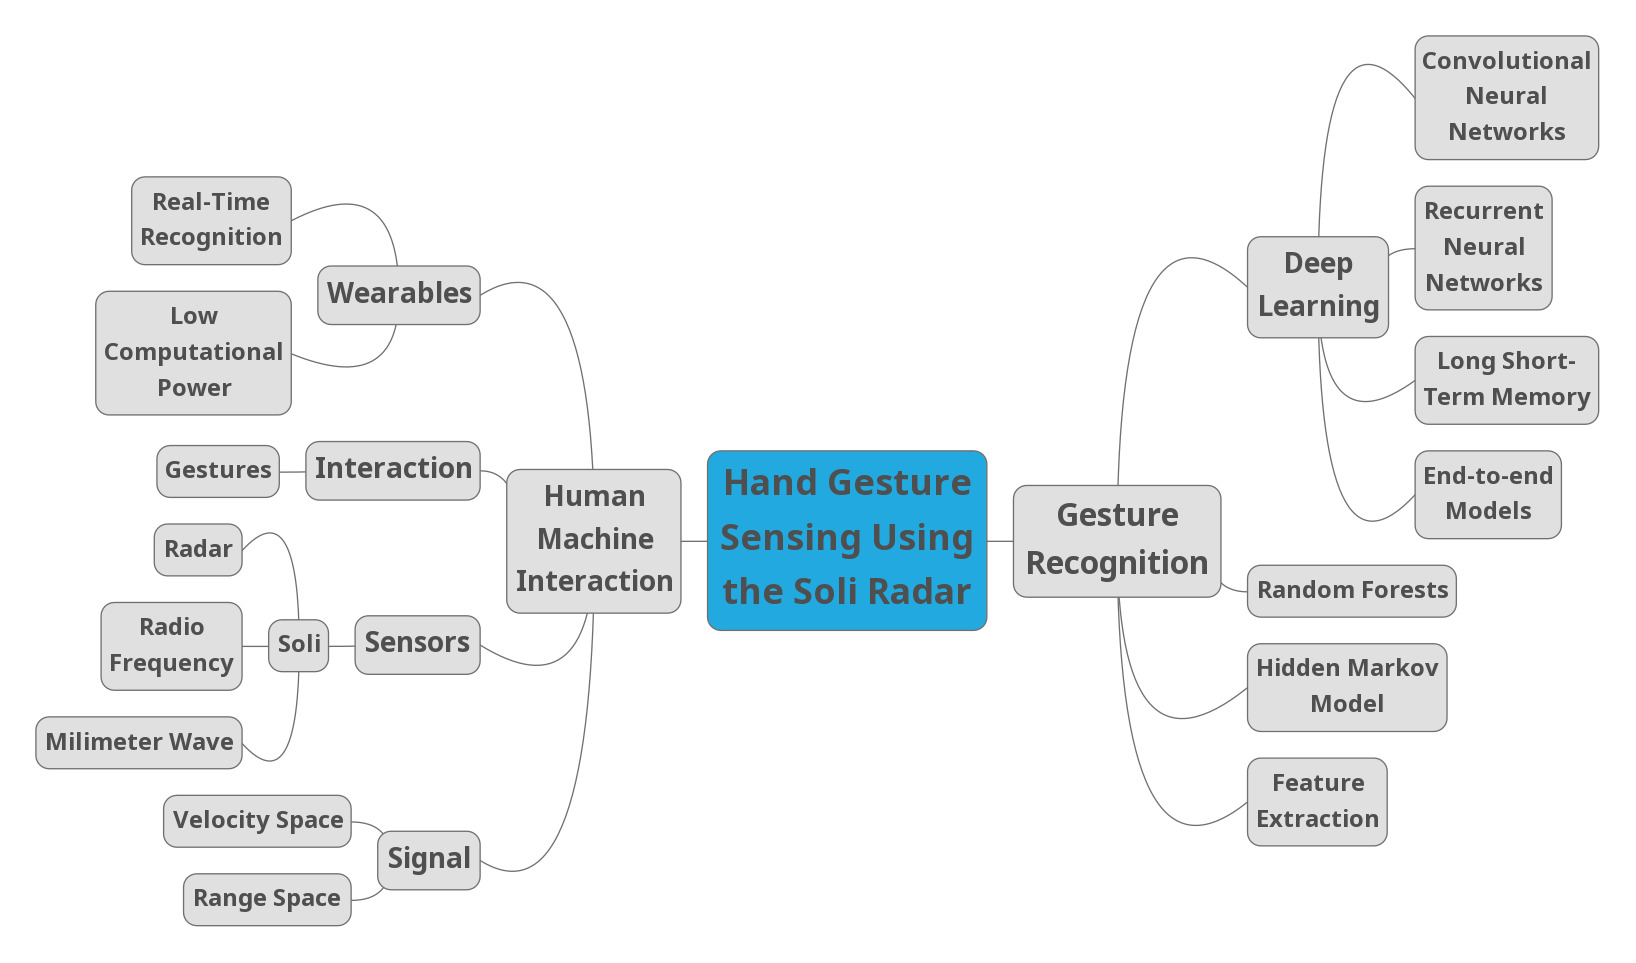
\includegraphics[width=1.25\textwidth]{mindmap_final.jpg}}
    \label{img:dsr0}
\end{figure} 
\end{center}

\newpage
\section{Descriptif de la recherche documentaire}
Pour construire la bibliographie, il a fallu, en premier lieu, cadrer notre sujet pour éviter de diverger du problème principal, nous nous sommes limité aux publications scientifiques portant sur la reconnaissance de gestes manuels en utilisant une technique radar en excluant d'autres types de données. Pour trouver nos sources, nous avons d’abord exploré les articles cités dans notre article principal. On a utilisé des moteurs de recherche comme Google Scholar, Web of Science, ACM et arXiv. Google Scholar renvoie une grande variété de documents, mais il ne met pas à disposition assez d’outils pour les filtrer, Web of Science, quant à lui, offre plus d'outils pour le filtrage et permet d'accéder aux textes complets en utilisant les abonnements de l'université. ACM et arXiv sont plus spécialisés en informatique, mais arXiv permet en plus d'accéder à des articles qui ne sont pas encore publiés et qu'il faut prendre avec précautions, car ils ne sont pas relus par les pairs. Pour les ressources qui sont exactement dans l'axe de notre sujet principal, on regarde les sujets cités par ceux-ci. On a procédé ainsi jusqu’à obtenir une base solide de connaissances pour pouvoir réaliser le projet. Pour construire notre bibliographie, on a utilisé le logiciel Mendeley qui permet d'importer les manuscrits directement depuis le navigateur, de gérer les références, de générer la bibliographie dans le format souhaité et rend possible le travail en groupe et en ligne.


\section{Bibliographie produite dans le cadre du projet}
 \nocite{*}
\printbibliography[heading=none]
\newpage
\section{Évaluation des sources}
Parmi les ressources cités, nous avons choisi les articles les plus importants pour notre
projet:

\subsection{Premier article \cite{Wang2016}}
Cet article est la ressource principale fournie par notre encadrant. Il a été publié en octobre 2016 dans « UIST '16: Proceedings of the 29th Annual Symposium on User Interface Software and Technology ». Le travail qui y est réalisé est pour nous la base de notre projet. Il a été cité 57 fois (source: ACM) et Il a été écrit par S. Wang, J. Song,O. Hilliges, J. Lien et I. Poupyrev, les trois premiers sont des chercheurs à l’ETH Zurich qui travaillent principalement sur les interactions homme-machine HCI, les deux derniers sont des chercheurs au Google ATAP qui ont développé le radar utilisé pour la recherche. Ils débutent leur article avec une revue de l’état de l’art en citant chaque source, ils proposent ensuite des modèles tout en testant leur performances. Cependant,  ils ont omis de présenter des tests détaillés sur la performance en temps de calcul et en mémoire. Tout leur travail est mis en accès libre sur Github (\url{https://github.com/simonwsw/deep-soli}). Le but de ce papier est de proposer un meilleur modèle pour la reconnaissance de gestes manuels que celui originellement proposé dans \cite{Lien2016}.


\subsection{Deuxième article \cite{Lien2016}}
Cette publication est le papier fondateur du radar Soli, elle est la source la plus citée dans notre article de base. Il est paru en juillet 2016 dans le journal « ACM Transactions on Graphics » qui est le journal dans le domaine de l’imagerie le plus revu par les pairs. Il est cité 150 fois (source: ACM). Ses auteurs sont: Jaime Lien, Nicholas Gillian, M. Emre Karagozler, Patrick Amihood, Carsten Schwesig, Erik Olson, Hakim Raja, Ivan Poupyrev qui sont tous membres de Google ATAP. L’article est de très bonne qualité, tout est expliqué en détails en fournissant les sources des informations. Tous les aspects du radar sont développés ainsi que les tests nécessaires. Ce travail a pour but de développer un radar adapté à la reconnaissance de gestes afin de l’intégrer dans le téléphone Google Pixel 4$^{\tiny{\textregistered}}$.


\subsection{Troisième article \cite{Simonyan2014}} 
\newline
Ce papier fait partie de nos ressources car il présente une architecture dont se sont inspirés les auteurs de \cite{Wang2016}. Il a été publié en janvier 2014 dans  « Advances in Neural Information Processing Systems » par Karen Simonyan et Andrew Zisserman qui sont tous deux chercheurs a l’université d’Oxford. Il a été cité 225 fois (Source: ACM). L’article n’est pas exactement dans notre axe de recherche mais nous tenons à le citer pour s’inspirer de leurs architectures. Le travail est fait avec rigueur, tout est expliqué en détails et des tests poussés sont effectués. 
\end{document}
